\documentclass[a4paper, 12pt, UTF8]{article}

\usepackage{xeCJK}
\setCJKmainfont[BoldFont={SimHei},ItalicFont={KaiTi}]{SimSun}

\usepackage{amsfonts}
\usepackage{amsmath}
\usepackage{graphicx}
\usepackage{indentfirst}
\usepackage{listings}
\lstset{
    columns=flexible,
    breakatwhitespace=false,
    breaklines=true,
    frame=single,
    numbers=left,
    numbersep=5pt,
    showspaces=false,
    showstringspaces=false,
    showtabs=false,
    stepnumber=1,
    rulecolor=\color{black},
    tabsize=2,
    texcl=true,
    escapeinside={\%*}{*)},
    extendedchars=false,
    mathescape=true,
}

\usepackage[colorlinks, citecolor=red]{hyperref}

\setlength{\evensidemargin}{-0.05in}
\setlength{\oddsidemargin}{-0.05in}
\setlength{\headheight}{-0.2in}
\setlength{\headsep}{0in}
\setlength{\textheight}{9.75in}
\setlength{\textwidth}{6.5in}
\setlength{\parindent}{2em}

\renewcommand{\baselinestretch}{1.5}

\begin{document}

\title{计算机视觉第5次作业}
\author{黎健成}
\date{2015210936}
\maketitle

% --------------------------------
\section{实验目的}

学习并掌握目标检测\textsuperscript{\cite{ref1}}。


% --------------------------------
\section{实验要求}

1. 安装Caffe\textsuperscript{\cite{ref2}}或Torch\textsuperscript{\cite{ref3}}

2. 使用RCNN\textsuperscript{\cite{ref4}}(或者Fast RCNN\textsuperscript{\cite{ref5}}, Faster RCNN\textsuperscript{\cite{ref6}})进行实验

% --------------------------------
\section{实验环境}

操作系统:Ubuntu 14.04.3 LTS

开发环境:gcc v4.7.3, MATLAB R2014b, Anaconda2-4.0.0


% --------------------------------
\section{实验问题}

给定一张图片,对其中的某些目标进行检测,输出相应的目标类别和包围盒(bounding box)。


% --------------------------------
\section{实验解决方案}

目标检测主要有四个基本步骤:

1. 候选区域生成(region proposal)

2. 特征提取(feature extraction)

3. 分类(classification)

4. 位置精修(rectangle refine)

在RCNN中,为4个步骤除了最后两个同时进行外均是依次进行;在Fast RCNN中,后3个步骤被统一起来;在Faster RCNN中,所有步骤都被统一到了一个深度网络框架内,大大提高了运行速度。这里主要使用Faster RCNN进行实验。

% ================================
\subsection{RCNN}

RCNN可以说是利用深度学习进行目标检测的开山之作,算法具体分为以下4个步骤:

1. 对每张图像生成大约2000个候选区域

2. 对每个候选区域,使用CNN提取特征

3. 特征输入每一类的SVM分类器进行类别判断

4. 使用回归器精细修正包围盒位置 

\subsubsection{候选区域生成}

使用Selective Search\textsuperscript{\cite{ref7}}方法从一张图像生成大约2000个候选区域,步骤如下:

1. 使用一种过分割手段,将输入的图像分割成小区域

2. 查看现有小区域,合并可能性最高的两个区域

合并的方法为:优先合并颜色(颜色直方图)相近的、纹理(梯度直方图)相近的、合并后总面积小的、合并后总面积在其包围盒中所占比例大的区域,且保证合并操作的尺度较为均匀以避免一个大区域陆续吞并其他小区域,保证合并后形状规则。

3. 重复第2步直到整张图像合并成一个区域位置

4. 输出所有曾经存在过的区域,即候选区域

\subsubsection{特征提取}

把输入的候选区域归一化成同一尺寸227×227。

使用在ILSVRC 2012\textsuperscript{\cite{ref8}}分类任务数据集预训练的AlexNet\textsuperscript{\cite{ref9}}卷积神经网络(CNN)进行调优(fine-tune),并把网络全连接层的输出提取作为特征。

\subsubsection{分类}

对每一个分类,训练一个线性SVM二分类器。之后可以使用这些分类器进行分类,即输入提取的特征,输出是否属于此类。

\subsubsection{位置精修}

目标检测问题的衡量标准是重叠面积,因此需要对包围盒的位置进行精细的修正。

对每一个分类,使用一个回归器(regressor)进行精修。使用分类正确与真实包围盒重叠面积大于0.6的候选区域作为训练样本,输入提取的特征,输出xy方向的缩放和平移。


% ================================
\subsection{Fast RCNN}

Fast RCNN方法解决了RCNN方法的三个问题:

1. 测试时速度慢

在RCNN中,每张图像内候选框之间大量重叠,提取特征操作冗余。
Fast RCNN将整张图像归一化后直接送入网络。在邻接时,才加入候选框信息,在末尾的少数几层处理每个候选框。

2. 训练时速度慢

在RCNN中,每张图像内候选框之间大量重叠,提取特征操作冗余。
Fast RCNN在训练时,先将一张图像送入网络,紧接着送入从这幅图像上提取出的候选区域。这些候选区域的前几层特征不需要再重复计算。

3. 训练所需空间大

在RCNN中,独立的分类器和回归器需要大量特征作为训练样本。
Fast RCNN把类别判断和位置精修统一用深度网络实现,不再需要额外存储。

\subsubsection{候选区域生成}

同RCNN。

\subsubsection{特征提取}

把输入的图像归一化为同一尺寸224×224直接送入网络。

在网络第5个阶段的卷积层后输入候选区域并连接到roi\_pool层。roi\_pool层在forward阶段将每个候选区域均匀分成$M \times N$块,对每块进行max pooling;在backward阶段中每个输入节点可能和多个候选区域的输出节点相连。

\subsubsection{分类}

在网络第5个阶段池化层输出的特征输入到cls\_score分类的全连接层中,输出一个$K + 1$维向量,表示K个分类和背景的概率。

\subsubsection{位置精修}

在网络第5个阶段池化层输出的特征输入到bbox\_predict调整包围盒的全连接层中,与分类层并行形成multi-task。输出一个$4 \times K$维向量,表示属于第K类的包围盒平移缩放的参数。


% ================================
\subsection{Faster RCNN}

在Faster RCNN中,区域生成网络(Region Proposal Network)代替Fast RCNN中的Selective Search方法,把4个步骤整合到一个网络中,加快了运行速度。


\subsubsection{候选区域生成}

使用一个区域生成网络(Region Proposal Network)来对输入的图片输出目标区域集及其相关分数。RPN本身是一个FCN(Fully Convolutional Network)。

对每一个大小为$W \times H$的feature map,考虑3种面积和3种比例共$k = 9$种候选区域(anchor),共$WHk$个anchor。

RPN训练的时候,对输入的每张图片,首先把每个标定的真值候选区域与其重叠比例最大的anchor记为前景样本;剩余的anchor中与某个标定重叠比例大于0.7的记为前景样本,而与任意一个标定的重叠比例都小于0.3的记为背景样本;最后剩余的anchor弃去不用。代价函数同时最小化分类误差和前景样本的区域位置偏差。

由于RPN和Fast RCNN都需要一个原始特征提取网络(raw feature extraction net),因此可以共享特征来加速。文中介绍了3种方法:

1. 轮流训练(Alternating training)。用$W_0$训练RPN并用RPN提取训练集上的候选区域。用$W_0$和候选区域训练Fast RCNN,参数记为$W_1$。再用$W_1$训练RPN并用RPN提取训练集上的候选区域……依此类推。

2. 近似联合训练(Approximate joint training)。合并成一个网络训练,在backward计算梯度时,把提取的roi区域当做固定值看待;在backward更新参数时,来自RPN和来自Fast RCNN的增量合并输入原始特征提取层。

3. 联合训练(Non-approximate joint training)。合并成一个网络训练,在backward计算梯度时,要考虑roi区域的变化的影响,具体参考\cite{ref10}。

\subsubsection{特征提取}

基本同Fast RCNN。

\subsubsection{分类}

基本同Fast RCNN。

\subsubsection{位置精修}

基本同Fast RCNN。


% ================================
\subsection{算法实现}

这里使用Faster RCNN进行实验。github上有相应的代码,我们把它下载下来再进行相应的安装和运行即可。

\begin{itemize}

\item 下载代码

\begin{lstlisting}[language={bash}]
git clone –recursive https://github.com/rbgirshick/py-faster-rcnn.git
\end{lstlisting}

\item 编译Cython模块

\begin{lstlisting}[language={bash}]
cd py-faster-rcnn
cd lib
make
cd ..
\end{lstlisting}

\item 编译Caffe and pycaffe

参考\url{http://caffe.berkeleyvision.org/installation.html}。

\begin{lstlisting}[language={bash}]
cd caffe-fast-rcnn
wget http://people.eecs.berkeley.edu/~rbg/fast-rcnn-data/Makefile.config
# 修改MATLAB\_DIR := /usr/local/MATLAB/R2014b
# 修改ANACONDA\_HOME := \$(HOME)/anaconda2
make -j8 && make pycaffe
cd ..
\end{lstlisting}

\item 下载预计算的Faster R-CNN检测器

\begin{lstlisting}[language={bash}]
./data/scripts/fetch_faster_rcnn_models.sh
\end{lstlisting}

\item 运行demo

\begin{lstlisting}[language={bash}]
./tools/demo.py
\end{lstlisting}

demo使用一个在PASCAL VOC 2007\textsuperscript{\cite{ref11}}目标检测任务预训练的VGG16网络,进行一些图片的目标检测。

\end{itemize}


% --------------------------------
\section{实验数据集}

\subsection{PASCAL VOC 2007数据集}

PASCAL VOC 2007数据集相关地址:\url{http://host.robots.ox.ac.uk/pascal/VOC/voc2007/index.html}

PASCAL VOC(Pattern Analysis, Statistical Modelling and Computational learning, Visual Object Classes) 2007指2007年一个视觉对象的分类识别和检测的挑战赛。挑战的主要目标是识别一些现实场景中的视觉对象类。数据集中有20个分类,分别是:

\begin{itemize}

\item 人:人

\item 动物:鸟、猫、牛、狗、马、羊

\item 交通工具:飞机、自行车、船、公共汽车、汽车、摩托车、火车

\item 室内物体:瓶子、椅子、餐桌、盆栽植物、沙发、电视/显示器

\end{itemize}

比赛主要分为分类、检测2个部分,这里我们只关注检测比赛。

检测比赛需要预测每个给定分类的目标标签(label)及包围盒(bounding box)。


% --------------------------------
\section{实验结果}

输出的log信息如下,可以看出,每张图片只需约0.1s即可预测出其中的所有目标及其包围盒。

\begin{lstlisting}
~~~~~~~~~~~~~~~~~~~~~~~~~~~~~~~~~~~
Demo for data/demo/000456.jpg
Detection took 0.136s for 300 object proposals
~~~~~~~~~~~~~~~~~~~~~~~~~~~~~~~~~~~
Demo for data/demo/000542.jpg
Detection took 0.121s for 160 object proposals
~~~~~~~~~~~~~~~~~~~~~~~~~~~~~~~~~~~
Demo for data/demo/001150.jpg
Detection took 0.108s for 192 object proposals
~~~~~~~~~~~~~~~~~~~~~~~~~~~~~~~~~~~
Demo for data/demo/001763.jpg
Detection took 0.117s for 203 object proposals
~~~~~~~~~~~~~~~~~~~~~~~~~~~~~~~~~~~
Demo for data/demo/004545.jpg
Detection took 0.135s for 300 object proposals
\end{lstlisting}

结果如图[\ref{figure_demo}]所示,可以看出,对于不同图像不同大小的目标,均能较好地得到其相应的包围盒;同一张图片也能在不同区域得到相应的目标包围盒。

\begin{figure}[ht!]
    \centering
    \begin{tabular}{cc}
        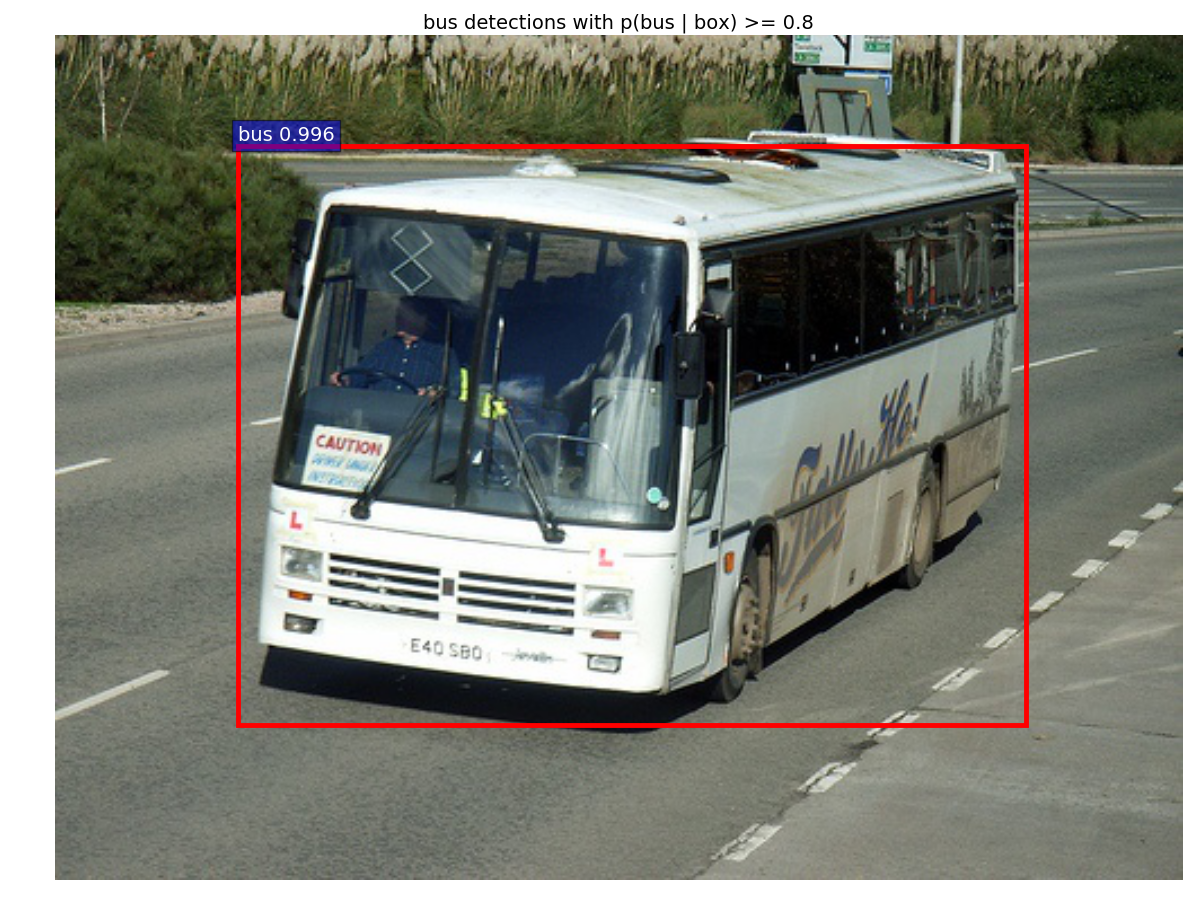
\includegraphics[width=0.36\textwidth]{figure_1.png} &
        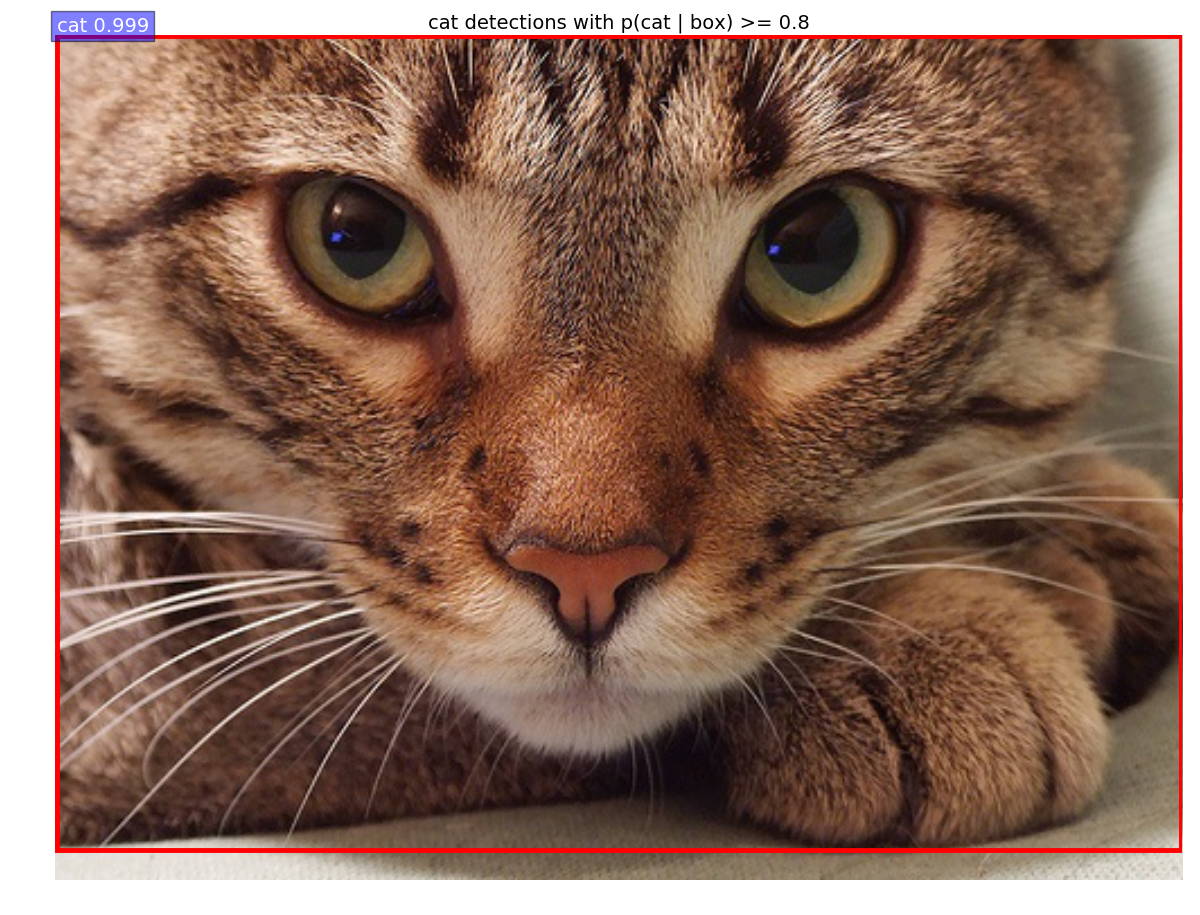
\includegraphics[width=0.36\textwidth]{figure_2.png} \\
        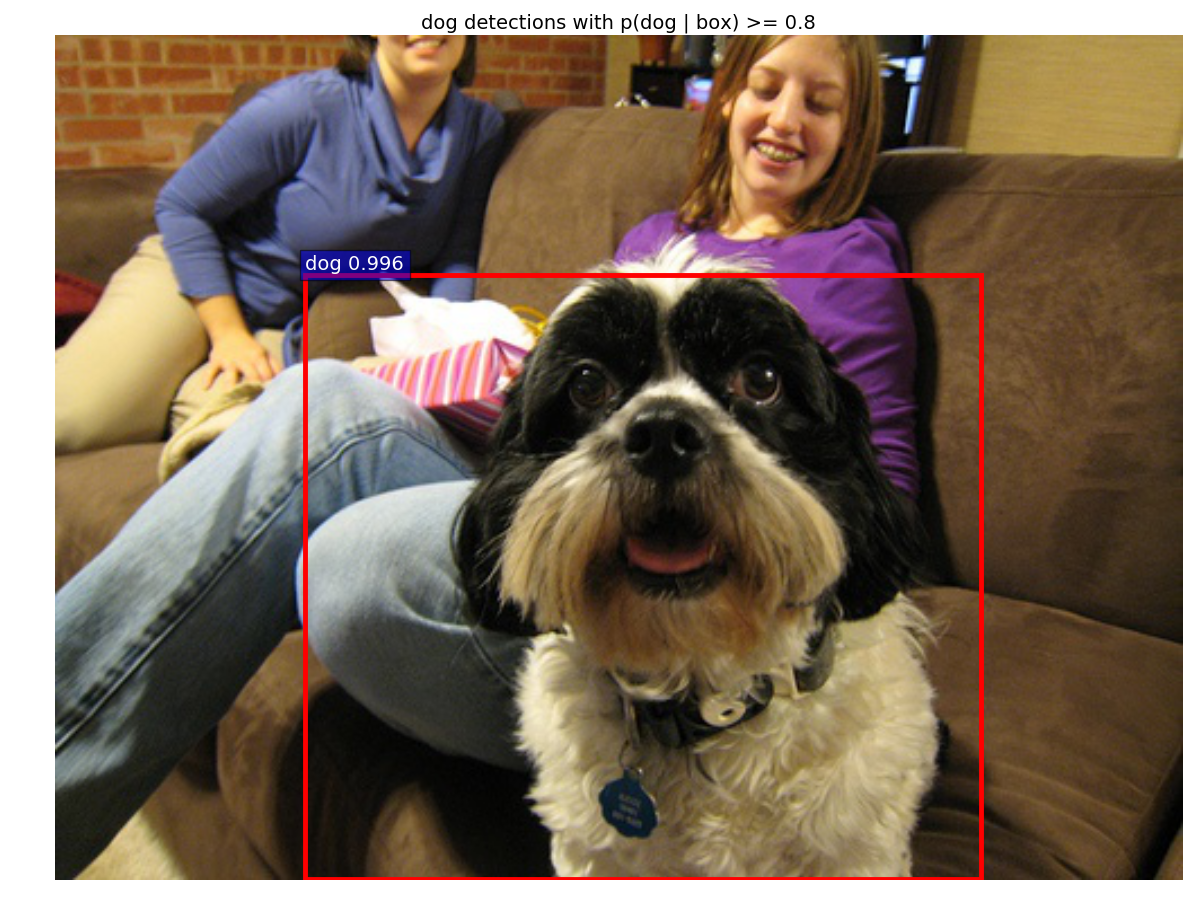
\includegraphics[width=0.36\textwidth]{figure_3.png} &
        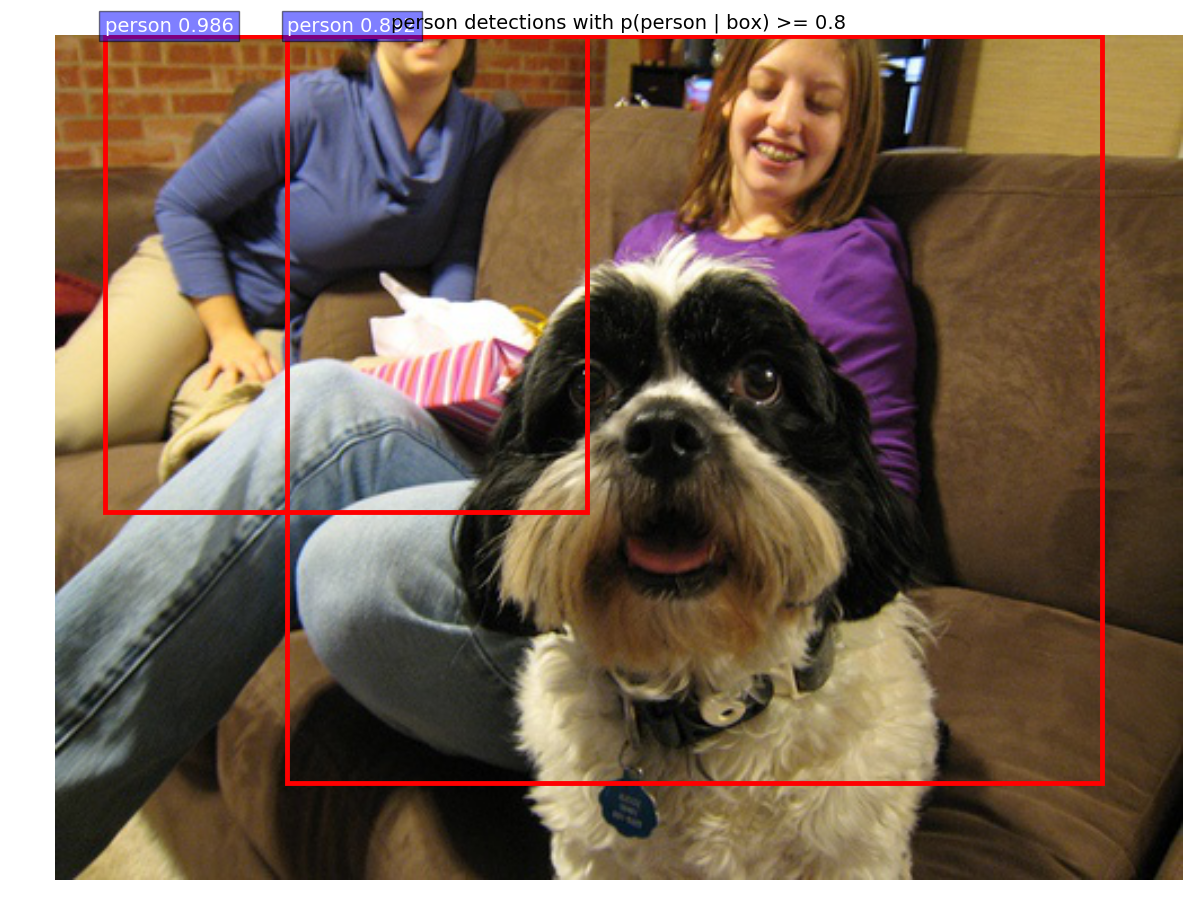
\includegraphics[width=0.36\textwidth]{figure_4.png} \\
        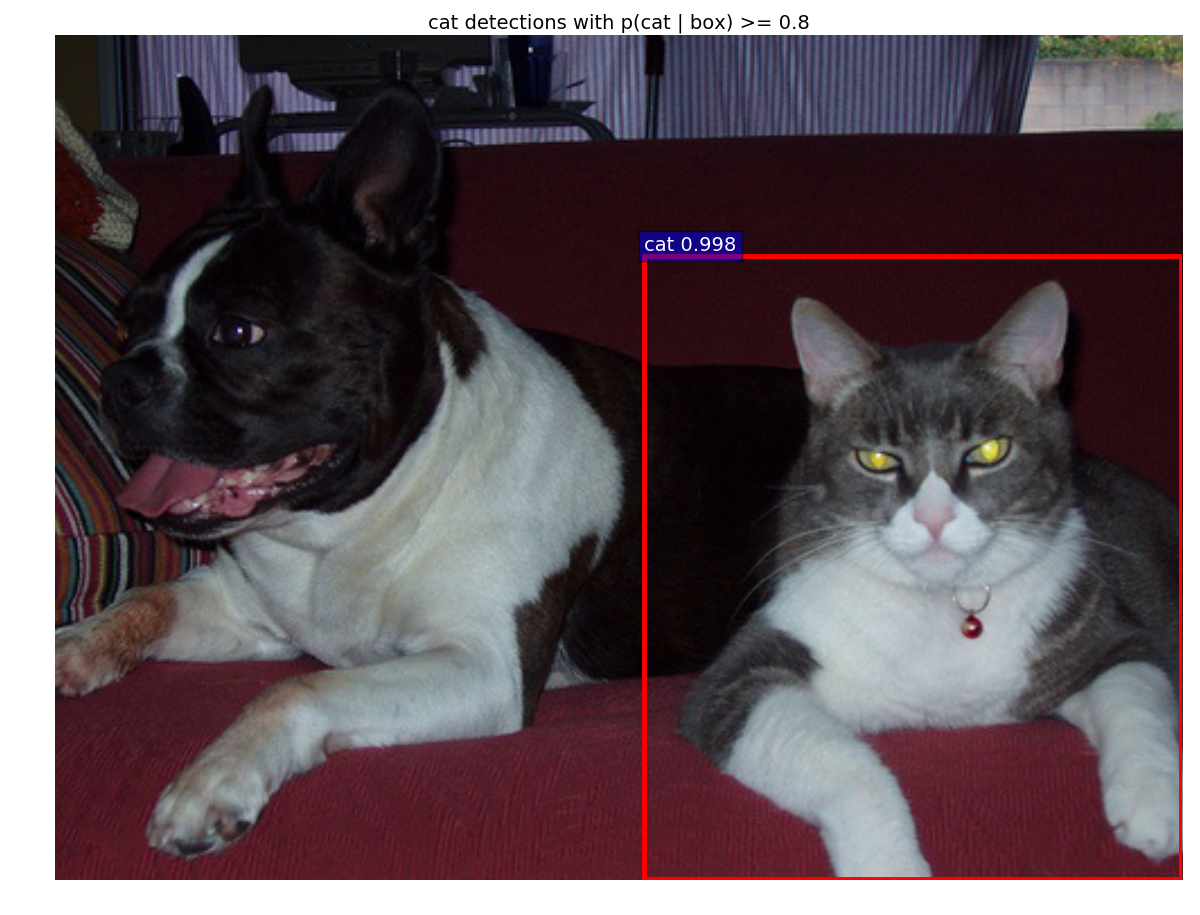
\includegraphics[width=0.36\textwidth]{figure_5.png} &
        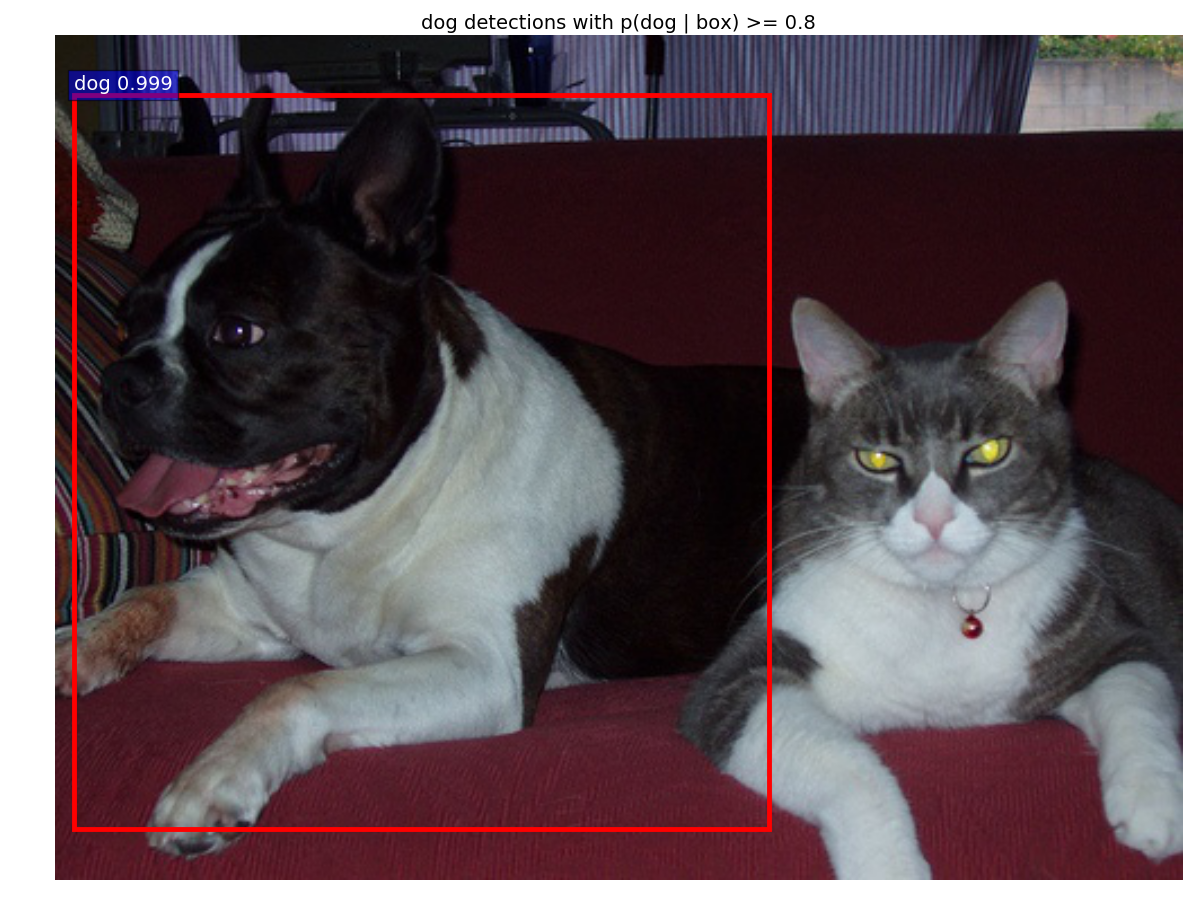
\includegraphics[width=0.36\textwidth]{figure_6.png} \\
        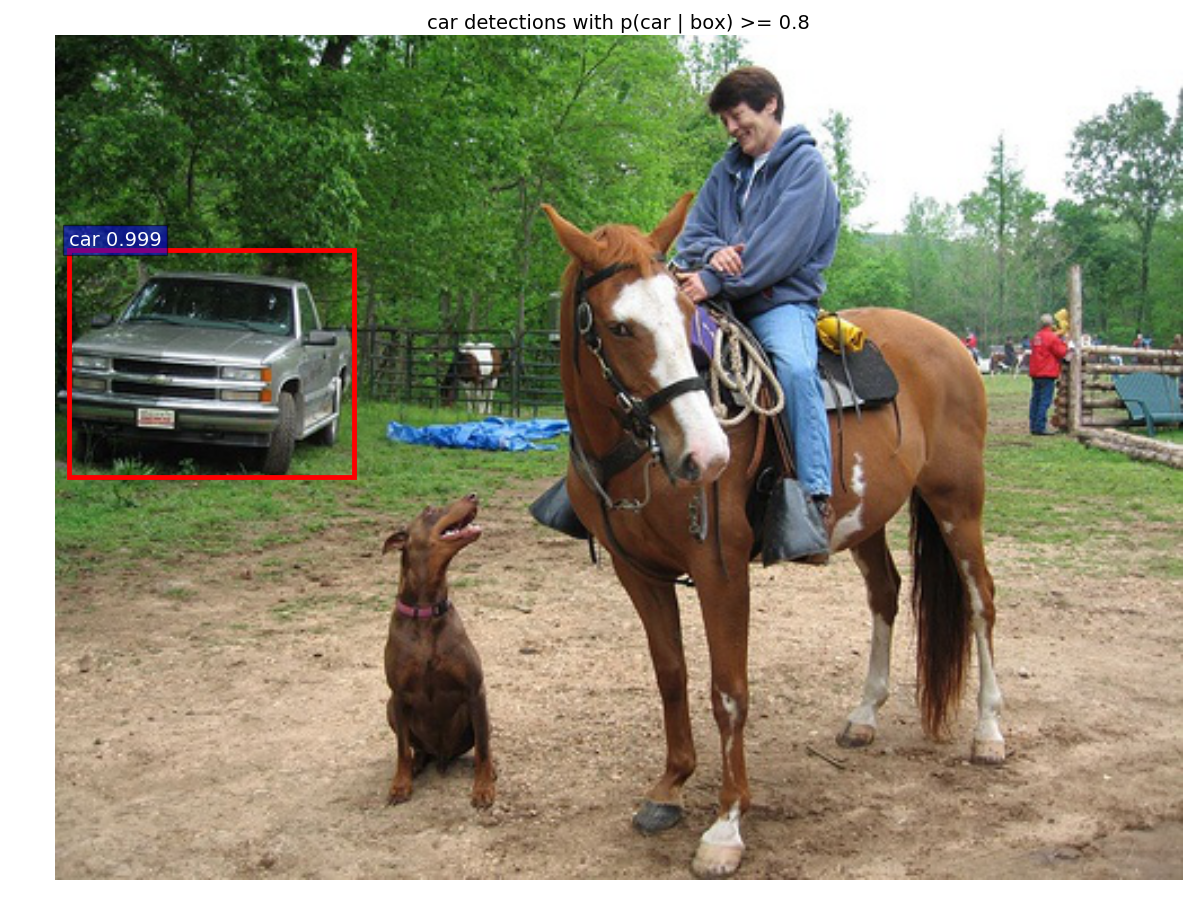
\includegraphics[width=0.36\textwidth]{figure_7.png} &
        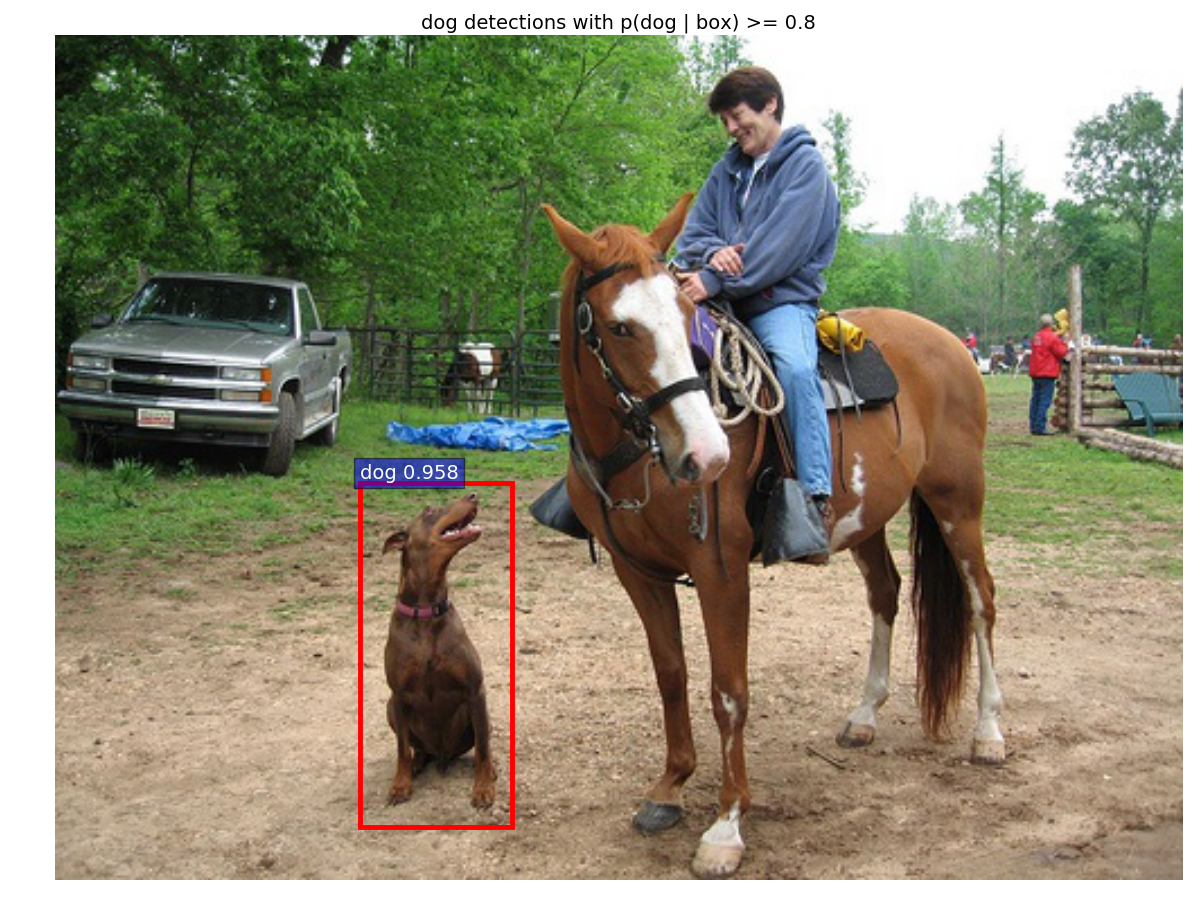
\includegraphics[width=0.36\textwidth]{figure_8.png} \\
        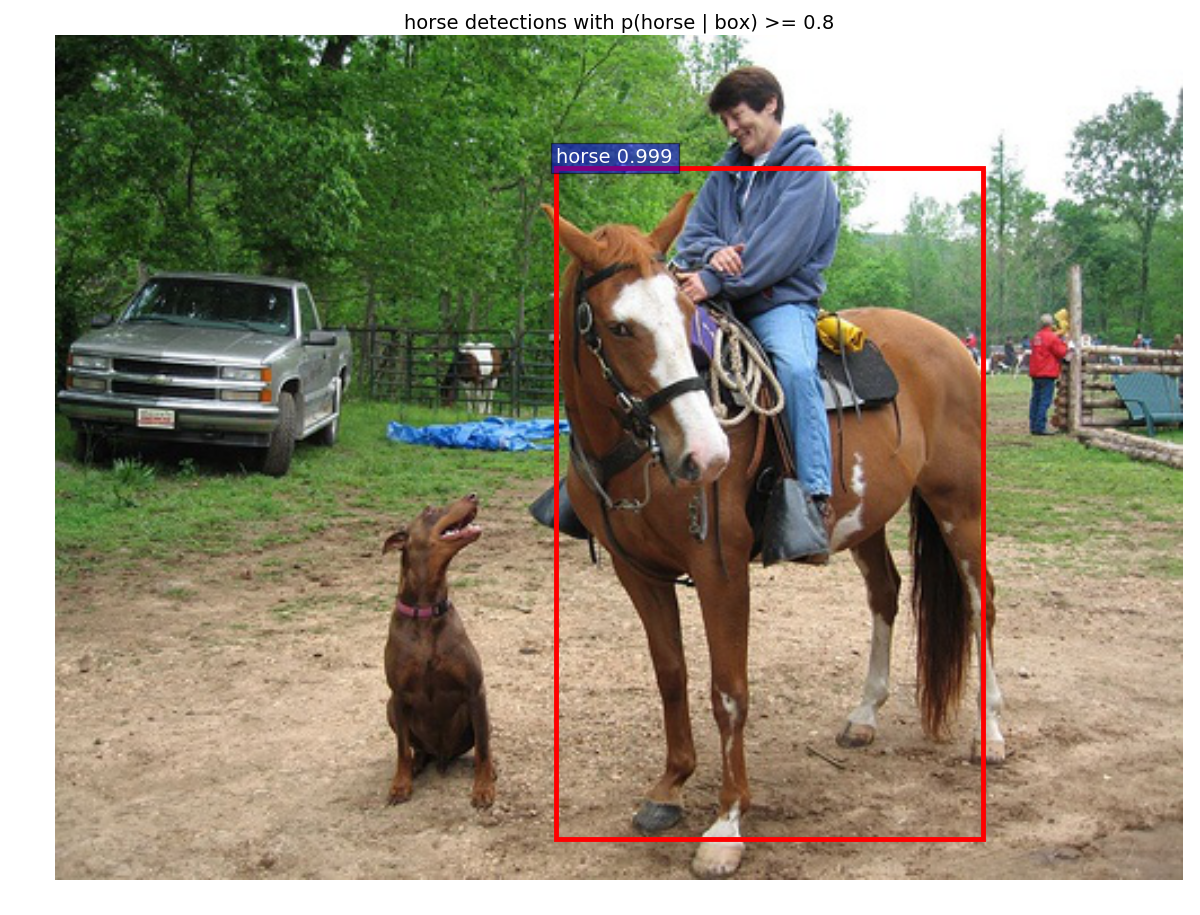
\includegraphics[width=0.36\textwidth]{figure_9.png} &
        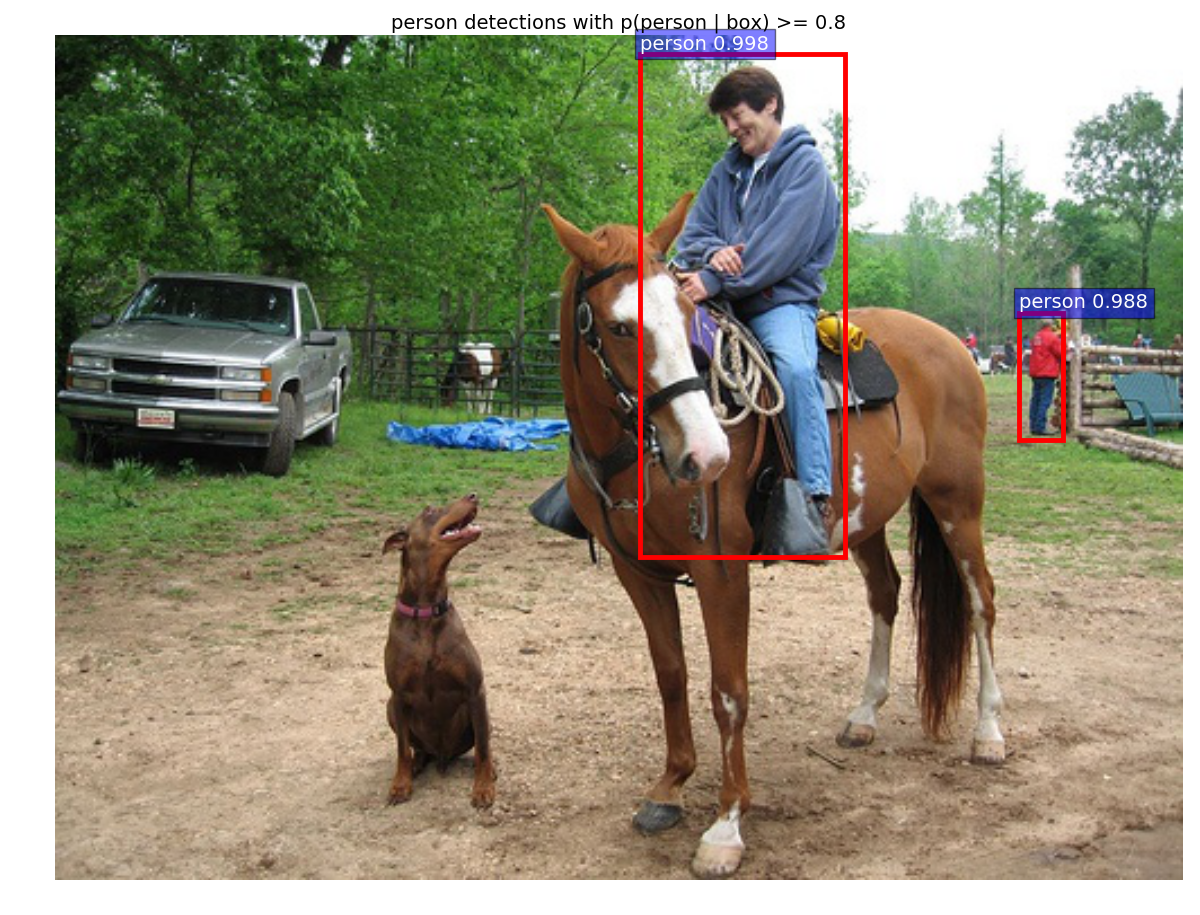
\includegraphics[width=0.36\textwidth]{figure_10.png} \\
    \end{tabular}
    \caption{demo结果}
    \label{figure_demo}
\end{figure}

% --------------------------------
\section{实验感想}

通过这次实验,熟悉了进行目标检测的RCNN、Fast RCNN和Faster RCNN这3种方法,并用Faster RCNN实现了目标检测,基本达到了实验目的。


% --------------------------------
\renewcommand{\refname}{参考}
\begin{thebibliography}{9}
\bibitem{ref1} Object detection. Wikipedia. 最后修订于2016年5月21日. \url{https://en.wikipedia.org/wiki/Object_detection}
\bibitem{ref2} Jia Y, Shelhamer E, Donahue J, et al. Caffe: Convolutional Architecture for Fast Feature Embedding[C]. ACM Multimedia, 2014.
\bibitem{ref3} Torch. Ronan, Clément, Koray and Soumith. \url{http://torch.ch/}
\bibitem{ref4} Girshick R, Donahue J, Darrell T, et al. Rich Feature Hierarchies for Accurate Object Detection and Semantic Segmentation[J]., 2014.
\bibitem{ref5} Girshick R. Fast R-CNN[C]. International Conference on Computer Vision, 2015.
\bibitem{ref6} Ren S, He K, Girshick R, et al. Faster R-CNN: Towards Real-Time Object Detection with Region Proposal Networks[C]. Neural Information Processing Systems, 2015.
\bibitem{ref7} Uijlings J, Sande K E, Gevers T, et al. Selective Search for Object Recognition[J]. International Journal of Computer Vision, 2013, 104(2): 154-171.
\bibitem{ref8} Russakovsky O, Deng J, Su H, et al. ImageNet Large Scale Visual Recognition Challenge[J]. International Journal of Computer Vision, 2014, 115(3): 211-252.
\bibitem{ref9} Krizhevsky A, Sutskever I, Hinton G E, et al. ImageNet Classification with Deep Convolutional Neural Networks[C]. Neural Information Processing Systems, 2012.
\bibitem{ref10} Dai J, He K, Sun J, et al. Instance-aware Semantic Segmentation via Multi-task Network Cascades[J]. Clinical Orthopaedics and Related Research, 2015.
\bibitem{ref11} The PASCAL Visual Object Classes Challenge 2007.  PASCAL2. \url{http://host.robots.ox.ac.uk/pascal/VOC/voc2007/index.html}
\end{thebibliography}

\end{document}
